\documentclass{beamer}
\usepackage{setspace}
\usepackage{gensymb}
\usepackage{caption}
%\usepackage{multirow}
%\usepackage{multicolumn}
%\usepackage{subcaption}
%\doublespacing
\singlespacing
\usepackage{csvsimple}
\usepackage{amsmath}
\usepackage{multicol}
%\usepackage{enumerate}
\usepackage{amssymb}
%\usepackage{graphicx}
\usepackage{newfloat}
%\usepackage{syntax}
\usepackage{listings}
%\usepackage{iithtlc}
\usepackage{color}
\usepackage{tikz}
\usetikzlibrary{shapes,arrows}



%\usepackage{graphicx}
%\usepackage{amssymb}
%\usepackage{relsize}
%\usepackage[cmex10]{amsmath}
%\usepackage{mathtools}
%\usepackage{amsthm}
%\interdisplaylinepenalty=2500
%\savesymbol{iint}
%\usepackage{txfonts}
%\restoresymbol{TXF}{iint}
%\usepackage{wasysym}
\usepackage{amsthm}
\usepackage{mathrsfs}
\usepackage{txfonts}
\usepackage{stfloats}
\usepackage{cite}
\usepackage{cases}
\usepackage{mathtools}
\usepackage{caption}
\usepackage{enumerate}	
\usepackage{enumitem}
\usepackage{amsmath}
%\usepackage{xtab}
\usepackage{longtable}
\usepackage{multirow}
%\usepackage{algorithm}
%\usepackage{algpseudocode}
\usepackage{enumitem}
\usepackage{mathtools}
\usepackage{hyperref}
%\usepackage[framemethod=tikz]{mdframed}
\usepackage{listings}
    %\usepackage[latin1]{inputenc}                                 %%
    \usepackage{color}                                            %%
    \usepackage{array}                                            %%
    \usepackage{longtable}                                        %%
    \usepackage{calc}                                             %%
    \usepackage{multirow}                                         %%
    \usepackage{hhline}                                           %%
    \usepackage{ifthen}                                           %%
  %optionally (for landscape tables embedded in another document): %%
    \usepackage{lscape}     


\usepackage{url}
\def\UrlBreaks{\do\/\do-}


%\usepackage{stmaryrd}


%\usepackage{wasysym}
%\newcounter{MYtempeqncnt}
\DeclareMathOperator*{\Res}{Res}
%\renewcommand{\baselinestretch}{2}
\renewcommand\thesection{\arabic{section}}
\renewcommand\thesubsection{\thesection.\arabic{subsection}}
\renewcommand\thesubsubsection{\thesubsection.\arabic{subsubsection}}

%\renewcommand\thesectiondis{\arabic{section}}
%\renewcommand\thesubsectiondis{\thesectiondis.\arabic{subsection}}
%\renewcommand\thesubsubsectiondis{\thesubsectiondis.\arabic{subsubsection}}

% correct bad hyphenation here
\hyphenation{op-tical net-works semi-conduc-tor}

%\lstset{
%language=C,
%frame=single, 
%breaklines=true
%}

%\lstset{
	%%basicstyle=\small\ttfamily\bfseries,
	%%numberstyle=\small\ttfamily,
	%language=Octave,
	%backgroundcolor=\color{white},
	%%frame=single,
	%%keywordstyle=\bfseries,
	%%breaklines=true,
	%%showstringspaces=false,
	%%xleftmargin=-10mm,
	%%aboveskip=-1mm,
	%%belowskip=0mm
%}

%\surroundwithmdframed[width=\columnwidth]{lstlisting}
\def\inputGnumericTable{}                                 %%
\lstset{
%language=C,
frame=single, 
breaklines=true,
columns=fullflexible
}


\begin{document}
\title{\textbf{JEE matrix problem through Python}}   
\author{\textit{Raktim Gautam Goswami (EE17BTECH11051) \newline Abhishek Bairagi (EE17BTECH11004)}} 
\date{\today} 

\frame{\titlepage} 

\frame{\frametitle{Table of contents}\tableofcontents} 


\section{Problem Statement} 
\frame{\frametitle{Problem Statement} 
Find the equation of the tangent to the circle, at the point 
\[\begin{bmatrix}
1\\
-1\\
\end{bmatrix}\]
whose centre is the point of intersection of the straight lines
\newline (2 1)\textbf{x} = 3
\newline (1 -1)\textbf{x} = 1
}


\section{Steps to solve} 
\frame{\frametitle{Steps to solve}
\begin{itemize}
\item \textbf{Find point of intersection of the two given lines}\newline\newline
\item \textbf{Find normal vector of the required tangent}\newline\newline
\item \textbf{Write in matrix format}\newline\newline
\end{itemize} 
}

\section{Solution}
\frame{\frametitle{Solution}
\begin{itemize}
\item \textbf{Finding point of intersection of the two given lines}
The given lines are 
\begin{equation}
$$ (2 1)x = 3$$
$$ (1 -1)x = 1$$
\end{equation}
This can be written as the matrix equation

\[ \left( \begin{array}{cc}
2 & 1 \\
1 & -1
\end{array} \right)
%
\left( \begin{array}{cc}
x
\end{array} \right)
\
%
 \begin{matrix}
=
\end{matrix} 
\
%
\left( \begin{array}{cc}
3\\
1
\end{array} \right)
\]
The point of intersection can be found by multiplying both sides of the equation by the inverse matrix.
\[\left( \begin{array}{cc}
x
\end{array} \right)
\
%
 \begin{matrix}
=
\end{matrix} 
\
%
\left( \begin{array}{cc}
1/3 & 1/3 \\
1/3 & -2/3
\end{array} \right)
%
\left( \begin{array}{cc}
3\\
1
\end{array} \right)
\]
\end{itemize} 
}
\section{Solution ...}


So the required intersection point is 
\[\left( \begin{array}{cc}
x
\end{array} \right)
\
%
 \begin{matrix}
=
\end{matrix} 
\
%
\left( \begin{array}{cc}
4/3 \\
1/3
\end{array} \right)
\]
The normal vector of the tangent will be the direction vector of the line joining the centre of circle C(4/3 , 1/3) and point of contact P(1,-1). So, the direction vector will be given by : C-P

\[\left( \begin{array}{cc}
4/3 \\
1/3
\end{array} \right)
\
%
 \begin{matrix}
-
\end{matrix} 
\
%
\left( \begin{array}{cc}
1 \\
-1
\end{array} \right)
%
 \begin{matrix}
=
\end{matrix}
%
\left( \begin{array}{cc}
1/3 \\
4/3
\end{array} \right)
\]

The equation of the line is of the form:

\[ \left( \begin{array}{cc}
1/3 \\
4/3
\end{array} \right)
%
\left( \begin{array}{cc}
X-P
\end{array} \right)
\
%
 \begin{matrix}
=
\end{matrix} 
\
%
\left( \begin{array}{cc}
0
\end{array} \right)
\]

Where P is 
\[ \left( \begin{array}{cc}
1 \\
-1
\end{array} \right)
\]






\section{Code}
\frame{\frametitle{Code}
The link of the code can be found here -
\href{https://github.com/abhishekbairagi/ee1390-/blob/master/Code/matrix.py}{Matrix code}
}


\section{Figure}
\frame{\frametitle{Figure}
The figure for the above problem from plotting is as follows.
\begin{figure}
  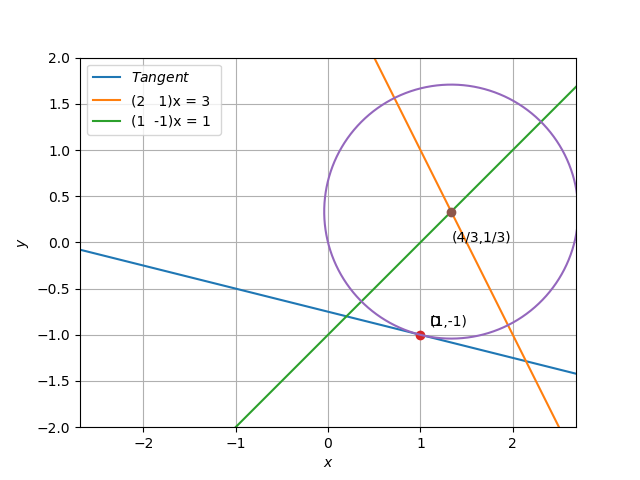
\includegraphics[width=200pt]{./Figs/Figure.png}
  \caption{Tangent on Circle}
  \label{figure}
\end{figure}
}

\end{document}
